\chapter{Round and Round We Go: Loops}

\begin{figure}[h!]
    \centering
    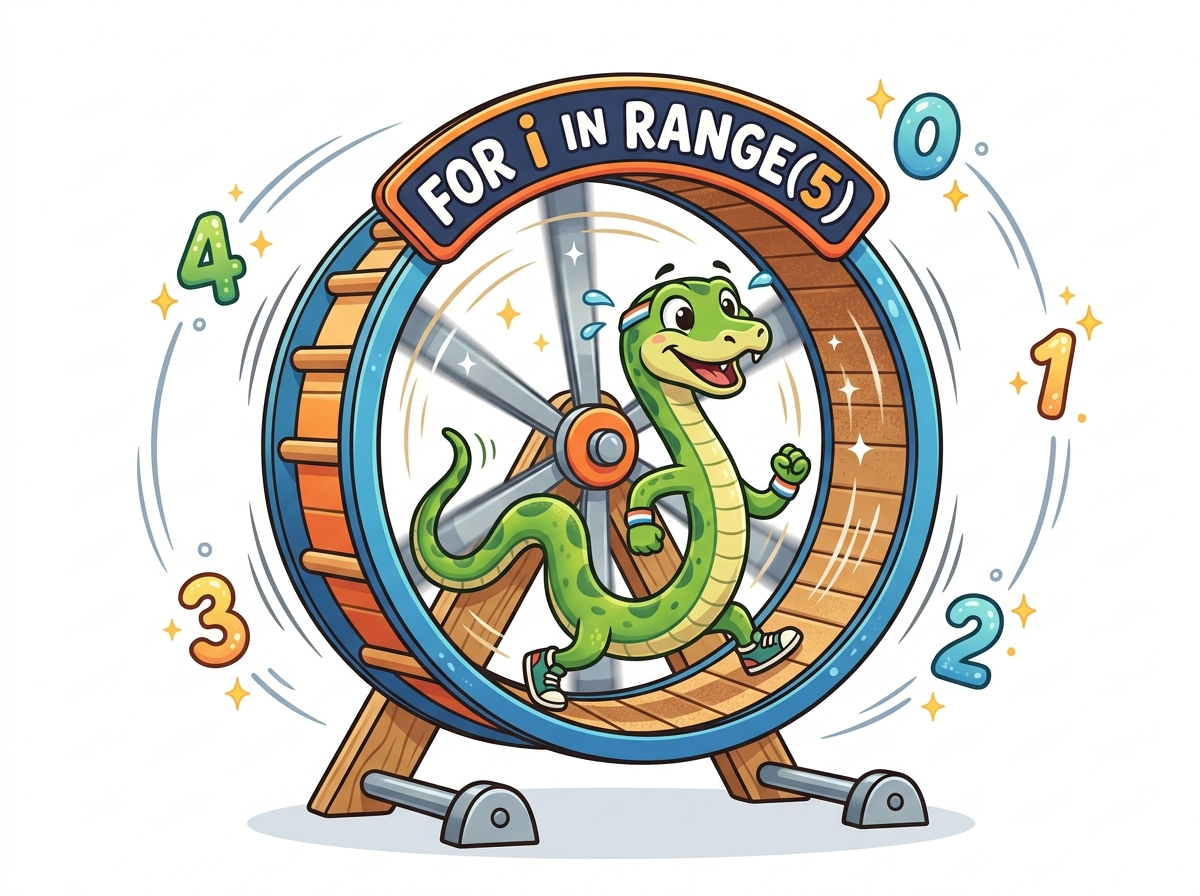
\includegraphics[width=0.75\textwidth]{images/ch3_hamster_wheel.jpg}
    \caption{Loops let your code repeat tasks like running on a hamster wheel without getting tired!}
\end{figure}

\section{Why Do Computers Love Repetition?}

If you ask a human to say ``I will not code in assembly'' 1,000 times, they will cry by iteration 14. If you ask Python to do it, it completes the task in 0.0002 seconds and asks for more!

In Python, we have two primary types of loops:
\begin{enumerate}
    \item \textbf{\texttt{for} loops:} Repeat a fixed number of times or iterate over items in a collection.
    \item \textbf{\texttt{while} loops:} Keep repeating as long as a condition stays \texttt{True}.
\end{enumerate}

\section{The Counting Wizard: \texttt{for} Loops \& \texttt{range()}}

The \texttt{range()} function is Python's number generator spell.

\begin{pycode}{Counting with range()}
# Count from 0 up to (but NOT including) 5
for i in range(5):
    print(f"Hamster wheel spin #{i}")

# range(start, stop, step)
print("Countdown:")
for count in range(10, 0, -2):
    print(f"{count}...")
print("BLAST OFF!")
\end{pycode}

\begin{chucklebreak}{Zero-Based Indexing}
Why does \texttt{range(5)} give us \texttt{0, 1, 2, 3, 4}? Because programmers start counting at zero! Why? Because in early memory architectures, index zero meant ``zero offsets from the beginning of the memory array''. Also, it keeps computer scientists feeling special.
\end{chucklebreak}

\section{The Relentless \texttt{while} Loop}

A \texttt{while} loop checks a boolean condition before every lap. If the condition is \texttt{True}, it executes the loop body. If it turns \texttt{False}, it stops.

\begin{pycode}{The Energy Counter}
energy = 3

while energy > 0:
    print(f"Coding... Energy left: {energy}")
    energy -= 1  # Equivalent to energy = energy - 1

print("Out of energy! Time for coffee!")
\end{pycode}

\begin{viperpitfall}{The Infinite Loop of Doom!}
If you forget to update your counter or condition inside a \texttt{while} loop:
\begin{lstlisting}[language=Python]
# DANGER: THIS WILL RUN FOREVER!
while True:
    print("I forgot to add an exit condition!")
\end{lstlisting}
If your terminal starts spinning out of control, press \texttt{CTRL + C} to break free!
\end{viperpitfall}

\section{Escape Hatches: \texttt{break} and \texttt{continue}}

- \textbf{\texttt{break}:} Instantly aborts the loop and jumps outside.
- \textbf{\texttt{continue}:} Skips the rest of the current lap and jumps straight to the next lap!

\begin{pycode}{Using break and continue}
for num in range(1, 10):
    if num == 3:
        print("Skipping 3 because it's unlucky!")
        continue
    if num == 7:
        print("Hit 7! Jackpot! Stopping loop.")
        break
    print(f"Processing item {num}")
\end{pycode}

\section{Code Example: Nested Loops Grid Generator}

Loops inside loops allow us to construct multi-dimensional grids, such as multiplication tables.

\begin{pycode}{Nested Loop Multiplication Table}
# Print a 4x4 multiplication table grid
print("--- 4x4 MULTIPLICATION TABLE ---")
for row in range(1, 5):
    row_text = ""
    for col in range(1, 5):
        product = row * col
        row_text += f"{product:4d}"  # Width of 4 spaces
    print(row_text)
\end{pycode}

\section{Practice Problems \& Exercises}

Loop around these 3 practice challenges!

\begin{snakelab}{Problem 3.1: The Classic FizzBuzz (Easy)}
Write a \texttt{for} loop that counts from $1$ to $20$.
\begin{itemize}
    \item If the number is divisible by $3$, print \texttt{"Fizz"}.
    \item If the number is divisible by $5$, print \texttt{"Buzz"}.
    \item If divisible by BOTH $3$ and $5$, print \texttt{"FizzBuzz"}.
    \item Otherwise, print the number itself!
\end{itemize}
\end{snakelab}

\begin{pycode}{Solution 3.1: FizzBuzz}
for n in range(1, 21):
    if n % 3 == 0 and n % 5 == 0:
        print("FizzBuzz")
    elif n % 3 == 0:
        print("Fizz")
    elif n % 5 == 0:
        print("Buzz")
    else:
        print(n)
\end{pycode}

\begin{snakelab}{Problem 3.2: Bank Vault PIN Retries (Medium)}
Write a \texttt{while} loop that simulates a bank vault security system with a max limit of $3$ attempts.
Simulate guesses starting with \texttt{1111}, \texttt{2222}, and ending with correct PIN \texttt{7777}.
Print access status for each attempt and abort early if correct!
\end{snakelab}

\begin{pycode}{Solution 3.2: Bank Vault Security}
correct_pin = "7777"
guesses = ["1111", "2222", "7777"]
attempt = 0
max_attempts = 3

while attempt < max_attempts:
    current_guess = guesses[attempt]
    attempt += 1
    print(f"Attempt {attempt}/{max_attempts}: Testing PIN '{current_guess}'...")
    
    if current_guess == correct_pin:
        print("SUCCESS! Vault opened!")
        break
    else:
        print("WRONG PIN!")
else:
    print("LOCKDOWN! Max attempts exceeded.")
\end{pycode}

\begin{snakelab}{Problem 3.3: Star Pyramid Pattern (Spicy)}
Write nested \texttt{for} loops to print an ascending pyramid of stars (\texttt{*}) with $5$ rows.
Row 1 has 1 star, Row 2 has 2 stars, ..., Row 5 has 5 stars.
\end{snakelab}

\begin{pycode}{Solution 3.3: Star Pyramid Pattern}
total_rows = 5

for row in range(1, total_rows + 1):
    stars = "*" * row
    print(stars)
\end{pycode}
